% !TeX root = OptCuts.tex

%\begin{algorithm}[h]
%\SetAlgoLined
%\KwData{$M$, $T^{k,i-1}$, $U^{k,i-1}$, $\delta^{k,i-1}$, $\lambda^{k+1}$}
%\KwResult{$T^{k,i}$, $U_a^{k,i-1}$}
%$\hat{\mathcal{E}}^{k,i-1}_T \leftarrow$ operationFiltering($M$, $T^{k,i-1}$, $U^{k,i-1}$); // Section~\ref{sec:operationFiltering}\\
%\For{each $e^{(k,i-1),j}_{T}$ in $\hat{\mathcal{E}}^{k,i-1}_T$}{
%  $\hat{f}_e(e^{(k,i-1),j}_{T}) \leftarrow \Big(E^j_s + \lambda^{k+1} \min_{U^{(k,i-1),j}} E_d(T^j,U)\Big) - L(T^{k,i-1},U^{k,i-1},\lambda^{k+1})$\;
%}
%$U_a^{k,i-1} \leftarrow U^{k,i-1}$\;
%\If{$\min_{e^{(k,i-1),j}_{T} \in \hat{\mathcal{E}}^{k,i-1}_T} \hat{f}_e(e^{(k,i-1),j}_{T}) \leq \delta^{k,i-1}$}
%{
%  $T^{k,i} \leftarrow T^j$, $U_a^{(k,i-1),j} \leftarrow \argmin_{U^{(k,i-1),j}} E_d(T^j,U)$\;
%}
%\caption{Topology Descent Step $(k+1,i)$}
%\label{alg:topologyStep}
%\end{algorithm}

\section{Coupled Discrete-Continuous Descent}
%\section{Coupled Topology and Distortion Descent}
\label{sec:topologySearch}
\danny{Did a pretty much full reworking of this section and the last two sections as well, if we're happy with this then we can clean up the pseudo code to make it consistent. Haven't touched the pseudocode yet.}
To perform our primal update, we seek to minimize the Lagrangian
%, composed of the weighted sum of seam-length, $E_s$ and distortion, $E_d$ jointly 
over both continuous changes in vertex position \emph{and} discrete changes in topology. 
%
To optimize over topology we could potentially perform exhaustive search over the graph of all possible mesh changes. This approach, however, clearly becomes intractable for any practical mesh size. 
Instead, we begin by recalling the standard process of optimizing a smooth energy solely over vertex DoFs. In such cases, each iterate generally forms a localized approximation of the minimized energy \justin{didn't understand previous phrase} and then uses it to propose a candidate direction for decrease. Then, since finding such a direction is expensive, we search along the proposed direction to ensure a significant decrease in energy (and not increase). 

Here, we extend this process to include explorations of discrete variations in topology. In analogy to seeking a continuous search direction, at the start of each new primal solve we will build many localized energy models to search in parallel for a likely candidate mesh operation to repeatedly propagate topology change, i.e., cutting or merging, over our UV mesh. Each inner iterate of the primal solve will successively apply this operation in combination with standard smooth descent to explore discrete-continuous descent until no further progress is made.% and so a primal update is found.    %<-- doesn't seem needed

\subsection{Energy Model}

At each outer iterate $k$, the Lagrangian for any proposed topology $T^i$ is  
\begin{align}
\ell(T^i) = \min_{U} L(T^i, U) = E_s(T^i) + \lambda^k \min_{U} E_d(T^i, U).
\end{align}
Then, for any valid topology changing operation, $o^{i,j}:T^i \rightarrow T^j$, the resultant change in energy is $\Delta \ell(o^{i,j}) = \ell(T^j) - \ell(T^i)$.

Starting from a known $(T^i, U^i)$, we approximate change in the Lagrangian by restricting the distortion update to the locally changed vertex stencil $U^{i,j}$ of the applied topological operation $o^{i,j}$ (see below for the stencils). 
We do this by holding all other remaining vertices $U_s$, shared in common with $T^i$, fixed in the mesh
to the same positions previously held in $U^i$, so that we have $U^j = (U^{i,j}, U_s)$.  Our approximate change in energy model is then 
%\danny{TODO: Still need some syntatic sugar to make this decomposition of fixed and free new vertices clean.}
\begin{align} 
d(o^{i,j}) = E_s(T^i) + \lambda^k \min_{U^{i,j}} E_d \big( T^i, (U^{i,j}, U_s) \big) - L(T^i,U^i,\lambda^k).
\end{align}

\subsection{Local Topological Operations}

We consider descent with topology changes propagated by three mesh operations.

\paragraph{Boundary Vertex Split}
Boundary vertices can be split along any interior incident edges. 
Each such candidate split generates two duplicate vertices forming the stencil to compute $d$.
\begin{wrapfigure}[5]{r}{0.4\linewidth}
  \begin{center}
  \vspace{-4mm}
    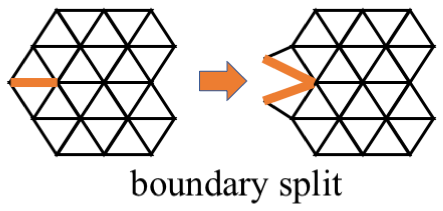
\includegraphics[width=1\linewidth]{fig/bSplit}
  \end{center}
\end{wrapfigure}
When splitting a boundary vertex along an edge connecting to another boundary vertex we either remove a hole or else produce a new chart in our UV map. For the latter case, we generate four duplicate vertices forming the stencil to compute $d$.
%\minchen{[TODO] 4-vertex merge to support joining two charts together, triangle moving operations?}

\paragraph{Interior Vertex Split}
\begin{wrapfigure}[4]{r}{0.4\linewidth}
  \begin{center}
  \vspace{-4mm}
    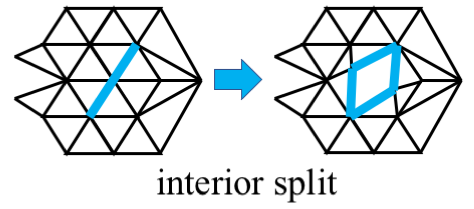
\includegraphics[width=1\linewidth]{fig/iSplit}
  \vspace{-1mm}
  \end{center}
\end{wrapfigure}
Interior vertices can be split along 
any pair of incident edges. Each such candidate split generates two duplicate vertices forming the stencil to compute $d$. 
%We ignore potential interior splits when this would be connected to an existing seam, as this is overloaded with propagating the boundary vertex split operation.

\paragraph{Corner Merge}
Corners are formed by three UV vertices corresponding to the tail edge of a cut seam on the input surface. 
\begin{wrapfigure}[5]{r}{0.4\linewidth}
  \begin{center}
  \vspace{-5mm}
    \includegraphics[width=1\linewidth]{fig/cMerge}
  \vspace{-4mm}
  \end{center}
\end{wrapfigure}
Merging the end vertices generates a single new vertex forming the stencil to compute $d$. Merging requires extra care here. Unlike vertex splitting, an initial location for the newly merged vertex must be selected. Na\"ive merging can violate local injectivity and so prevent progress if we are working with barrier-type energies like symmetric Dirichlet. We initialize a merged vertex to the average of its parent vertices. If inversion is detected, we then apply Agmon's relaxation~\shortcite{Agmon1954Relaxation} to iteratively project to an inversion-free position. On rare occasions this will not suffice and so we remove the proposed operation from our queue; see below.
%However, cases are still there when only moving the merged vertex is not enough to obtain an inversion free initial local stencil. In these situations, we will just abandon the candidate. This rarely happens in practice and does not affect our result.\justin{didn't follow the last two sentences, maybe needs a small figure}

\subsection{Topology Search Candidates}
\label{sec:descent_op}
In analogy to a continuous search direction, at the start of each new primal solve we search for a candidate mesh operation to propagate descent. 
%
To select the candidate mesh operation we first consider all $m$ boundary vertices in the current topology $T^k$. \danny{Minchen: confirm this detail:} For each such vertex we compute the standard deviation over all the distortion energy gradients acting on the vertex contributed from incident elements. From the set of $m^{0.8}$ boundary vertices with largest deviation we then build a set of candidate mesh operations $O^k$ formed by boundary vertex splits and corner merges (when valid) on those vertices. \minchen{The filtering is only applied on split operations, not on corner merge. We simply query all corners, there's not many of them, and the filtering criteria for splits is not appropriate for merge.} We then find a minimizer
\begin{align}
\label{eq:minO}
o^{i,j} = \argmin_{o \in O^k} d(o).
\end{align}
With local support, all queried $d$ in this minimization can be evaluated in parallel. If the minimizing operation promises descent, i.e., $d(o^{i,j}) < 0$, we set our candidate mesh operation for our descent process, $s^k$, with this operation, $s^k \leftarrow o^{i,j}$. Otherwise, we go on to find the $(n-m)^{0.8}$ interior vertices with largest deviation and rebuild $O^k$ as the set of all interior vertex splits on those vertices. A $d$ minimizing interior split operation $o^{i,j} \in O^k$, again using (\ref{eq:minO}), is then set as the set $s^k \leftarrow o^{i,j}$ for our descent process.

\subsection{Iterated Search, Propagation and Descent}

Once we have computed our candidate search operation $s^k$, we begin an inner loop iteration, indexed by superscript $i$ (recalling outer iterates are indexed by $k$), to solve the primal variable update. At the start of this process we initialize our desired upper bound on estimated decrease to $\delta^0 = 0$; this will be updated at each successive iterate. Then, each inner iteration $i$ proceeds by first propagating topology change followed by smooth coordinate update. 

Each topology propagation step first generates a set of all possible mesh operations $\mathcal{E}(s^k, T^{i-1})$ that could continue to propagate the seed operation $s^k$ on topology $T^{i-1}$, e.g. all edges that could continue to propagate a boundary splitting cut from the current tail. See Figure\ \ref{fig:propagation} for illustrations on how we propagate each operation.
As in seeking our seed operation we once again find the $d$-minimizing operation from this small set of candidate operations
\begin{align}
\label{eq:minE}
o^{i,j} = \argmin_{o \in \mathcal{E}(s^k)} d(o).
\end{align}
If this minimizer provides sufficient estimated decrease, so that $d(o^{i,j}) < \delta^{i-1}$, we accept the topology update setting $T^i \leftarrow T^j$; otherwise, we keep topology unchanged with $T^i \leftarrow T^{i-1}.$

\begin{figure}[t]
\centering
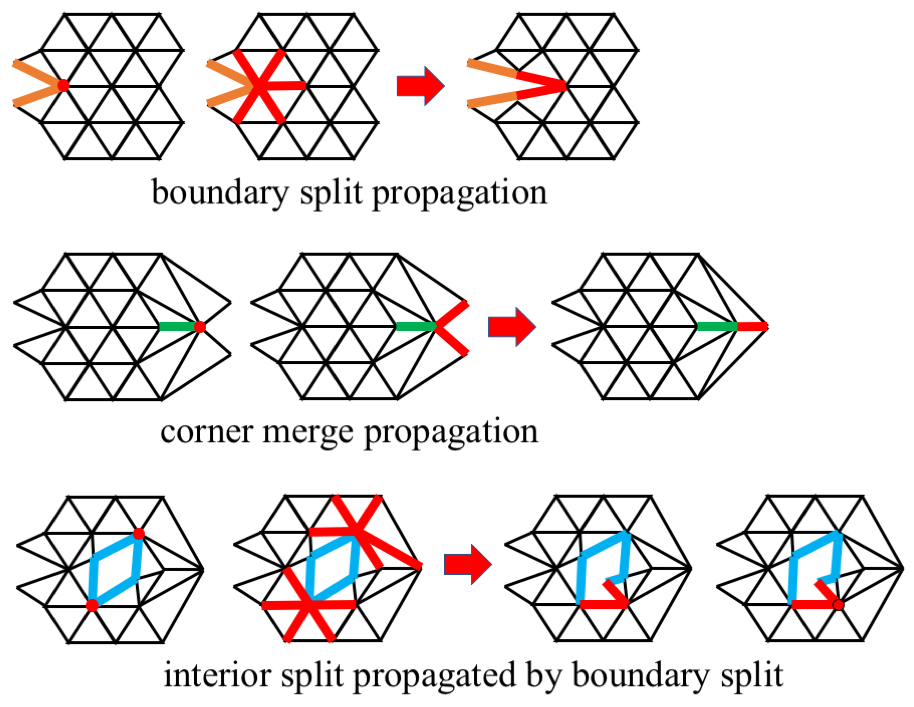
\includegraphics[width=0.8\linewidth]{fig/propagation.png}
\caption{Propagation of boundary split (orange), corner merge (green), and interior split (blue). When propagating boundary split, all edges that could continue to propagate a boundary splitting cut from the current tail would be considered (a); for corner merge we just query the new corner at the current tail (b); for interior split, once an incident edge of either the two tail is splitted as propagation, in the following iterations it would be the same as propagating boundary split (c).}
\label{fig:propagation}
\end{figure}

The subsequent coordinate update then simply applies a single step of projected Newton descent with line search to update the vertex coordinates $U^i$; see Section~\ref{sec:descentStep} for details. We then ask for the next topology update to gain similar or greater magnitude decrease by setting $\delta^i = E_d(U^i) - E_d(U^{i-1})$.

This process terminates at iteration $i+1$ when smooth iterations have converged (either by gradient or relative error norm) \emph{and} the propagation of the seed mesh operation produces no further descent. We then set $(T^k,U^k) \leftarrow (T^{i+1},U^{i+1})$ and begin the next outer iterate $k+1$ with the dual variable update. 


